% \FloatBarrier

\section{Evaluation}
\label{sec:evaluation}


\begin{figure*}[htbp]
  \centering
  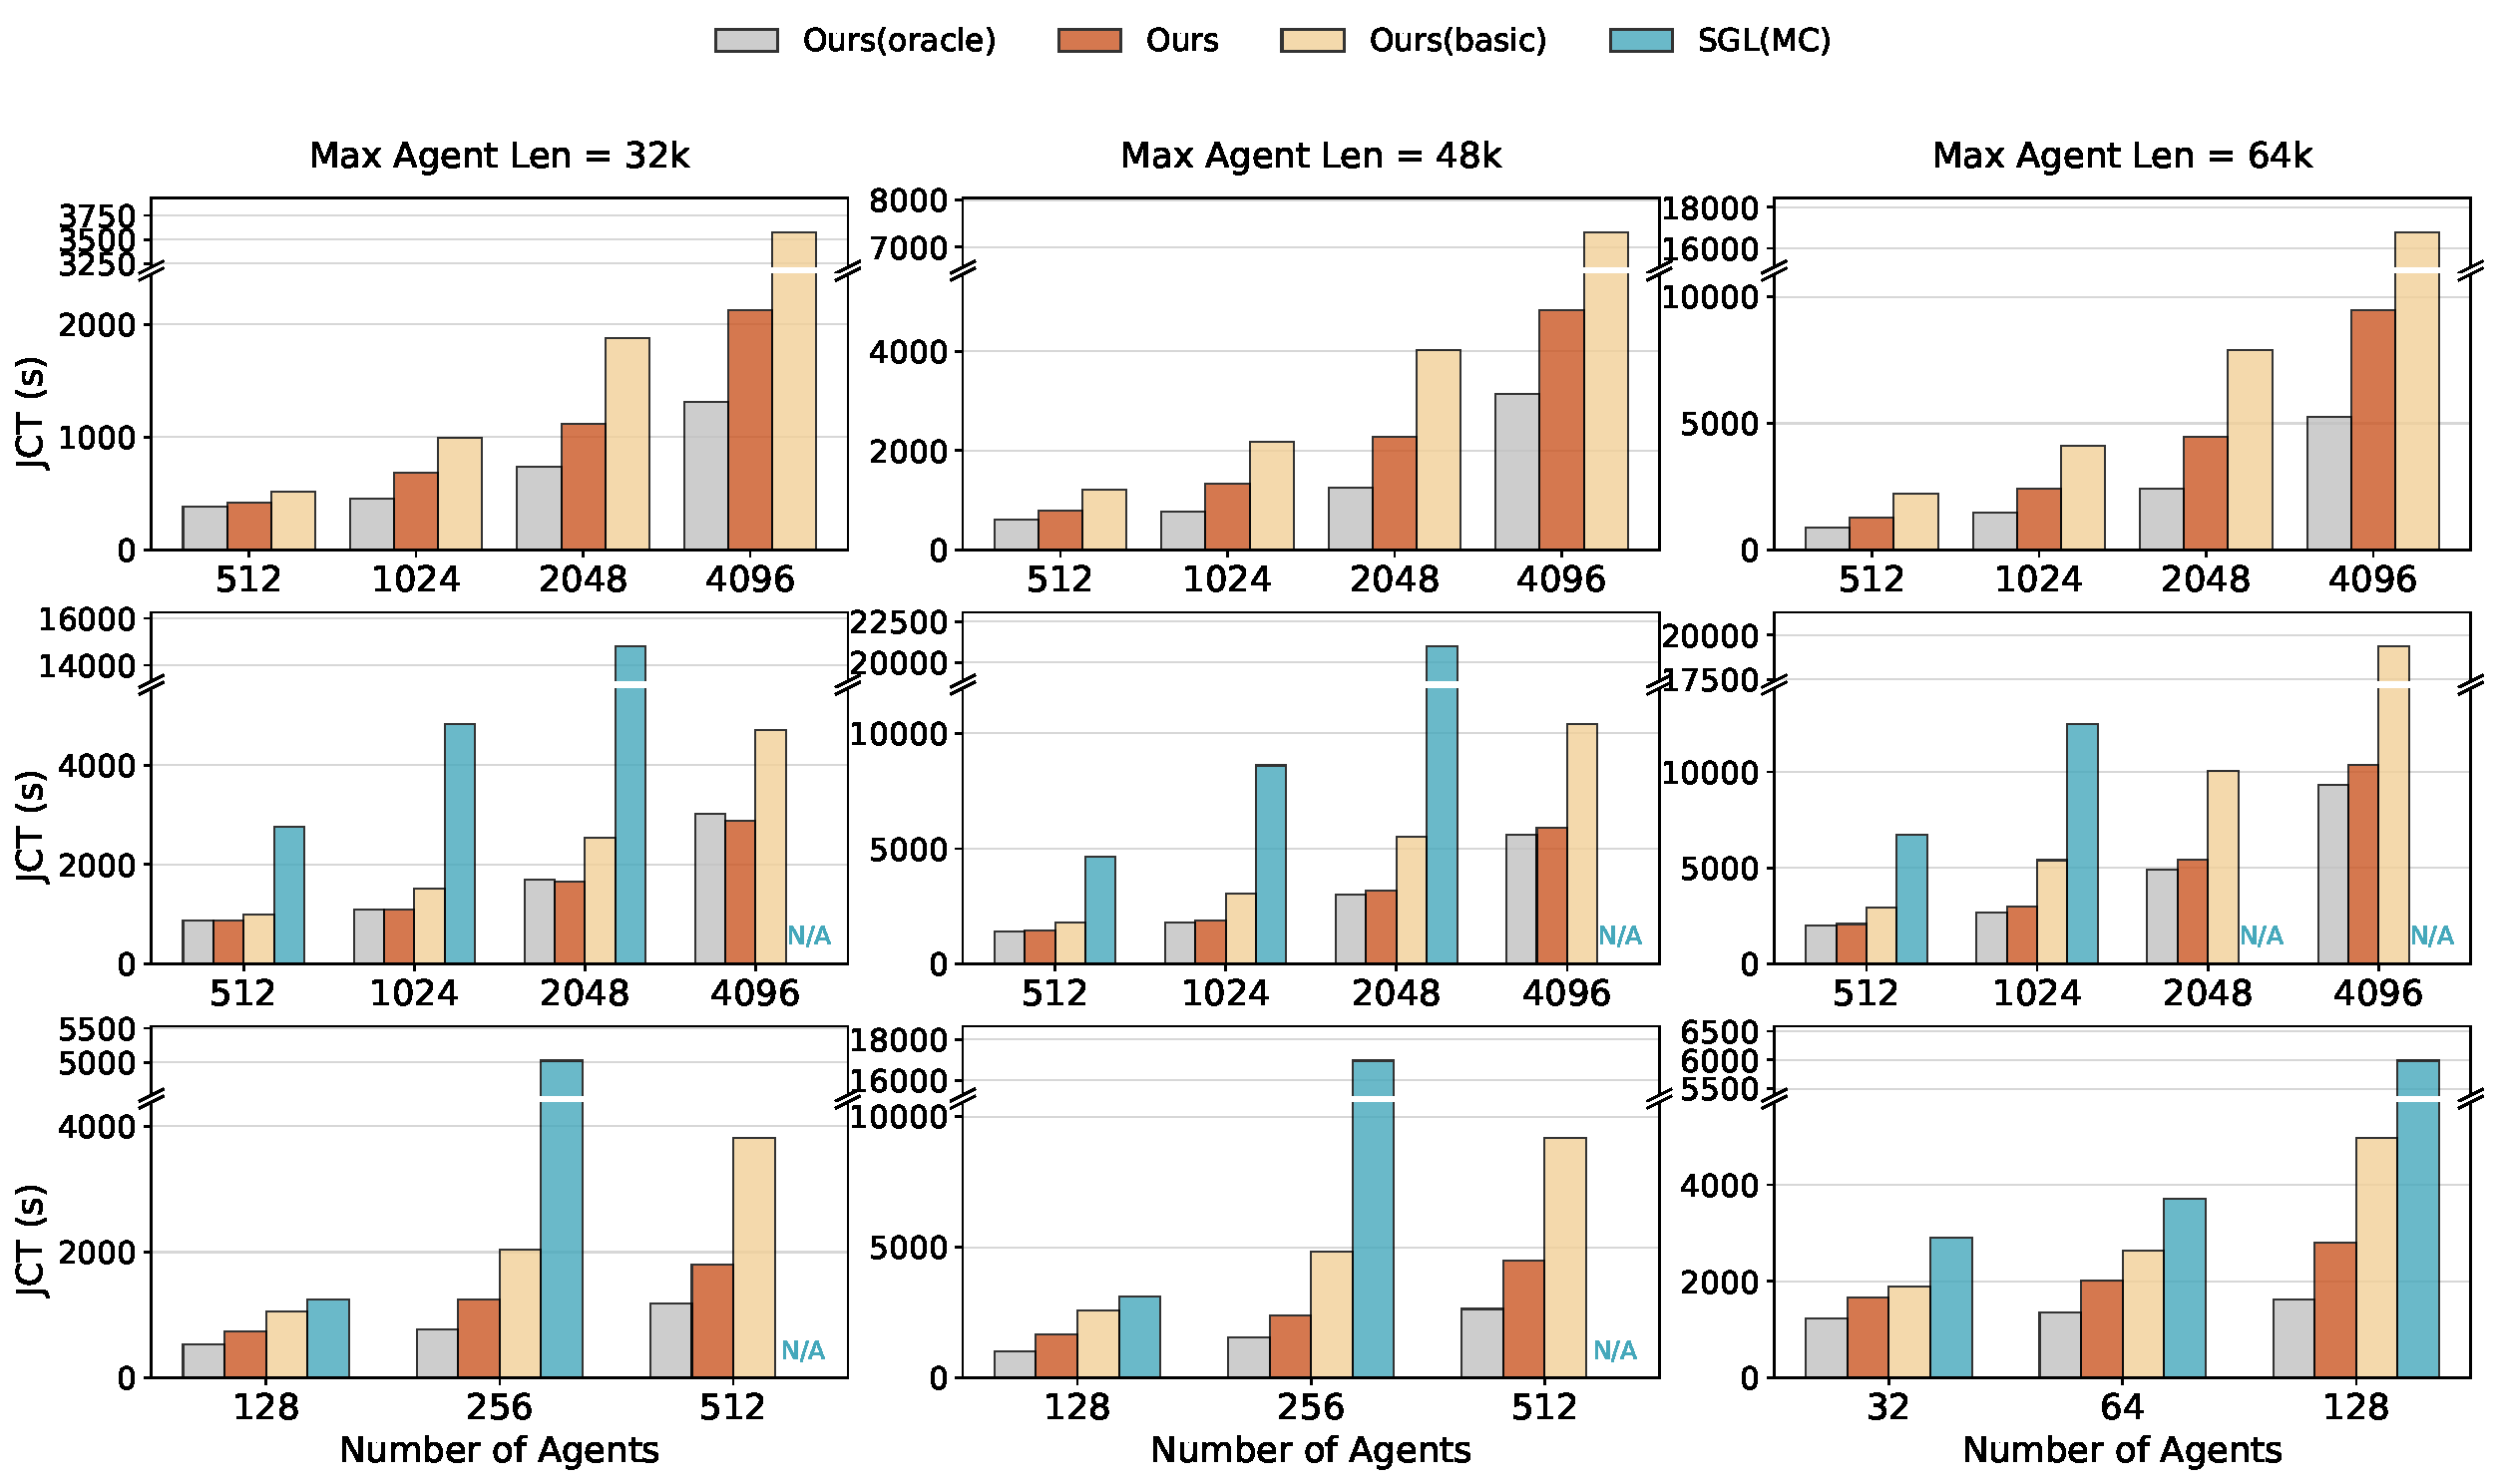
\includegraphics[width=0.98\linewidth]{figures/rollout_combined}
  \caption{\normalfont Offline inference performance under varying numbers of agents and maximum agent context lengths. Top: DS 27B. Middle: DS 660B. Bottom: Qwen 32B. N/A for running into an error before finishing.}
  \label{fig:rollout}
\end{figure*}


\subsection{Implementation}
\label{subsec:impl}
We implement \sysname based on our in-house inference framework.
For CUDA kernels, our in-house framework adopt the combination of FlashMLA \cite{FlashMLA}, DeepGEMM \cite{DeepGEMM}, and DeepEP \cite{DeepEP}, which aligns with the current mainstream open-source framework \cite{NIPS24:SGLang, SOSP23:PagedAttention}.
The \sysname implementation involves approximately 5K lines of modifications on top of it.
We adopt 3FS \cite{3FS} as distributed storage and use an \verb|io_uring|-like interface for kernel bypass.

\subsection{Experimental Setup}
\label{subsec:experimental-setup}

\paraf{Testbed.}
We conduct our experiments on a cluster of GPU servers with InfiniBand interconnection. Each server has 8 NVIDIA Hopper GPUs and dual processors. Additionally, each node is provisioned with eight 400Gbps RDMA NICs connected to InfiniBand network and one additional storage NIC connected to 3FS. The computation and storage networks are physically isolated. Our cluster-wide 3FS has no internal DRAM cache and can saturate the 400Gbps bandwidth of the storage NIC.

\parabf{Models.}
We evaluate on three models: (1) DeepSeek V3.2 \cite{DeepSeekV32} 660B, an MoE model with DeepSeek Sparse Attention, denoted as \emph{DS 660B}, (2) a 27B downscaled version of DS 660B, denoted as \emph{DS 27B}, and (3) Qwen2.5-32B \cite{qwen2025qwen25technicalreport}, a dense model with GQA, denoted as \emph{Qwen 32B}.
DS 660B and Qwen 32B correspond to the publicly released checkpoint on HuggingFace.
DS 27B is our internal experimental model with a similar architecture to DS 660B.
Detailed specifications are provided in \autoref{sec:27b-model-specs}.


\parabf{Datasets.}
We collected three agent trace datasets from our production agentic RL training workloads with varying maximum context lengths (MaxLen). Each dataset contains 500 trajectories. The average interaction turns (Turns), average appended and generated tokens per turn (Append and Gen), average number of total tokens (Total), and average number of context tokens (Context) are summarized in \autoref{tab:agent-dataset-statistics}. 

\begin{table}[t!]
\centering
\caption{\normalfont Statistics of agent trace datasets.}
\begin{tabular}{cccccc}
\toprule
\textbf{MaxLen} & \textbf{Turns} & \textbf{Append} & \textbf{Gen} & \textbf{Total} & \textbf{Context} \\
\midrule
32K  &  60 & 608  & 148 & 28639 & 17183 \\
48K  & 106 & 474  & 172 & 42607 & 25120 \\
64K  & 157 & 429  & 176 & 55958 & 32721 \\
\bottomrule
\end{tabular}
\label{tab:agent-dataset-statistics}
\end{table}


\parabf{Baselines.}
We compare \sysname, denoted as Ours, against the following baselines:

\begin{itemize}[leftmargin=*]
\item \textbf{SGL(MC)}: SGLang \cite{NIPS24:SGLang} (commit 19089aa) with HiCache \cite{Hicache}, Mooncake \cite{FAST25:Mooncake} Store enabled and 3FS as the storage backend, and Mooncake Transfer Engine for prefill-decode disaggregation.
We did not run SGL(MC) for DS 27B because SGLang lacks support for this downscaled version.
\item \textbf{Basic}: Our unmodified internal inference framework (detailed in \autoref{subsec:impl}).
Comparing \sysname and SGL(MC) is unfair due to implementation differences.
Therefore, we only report performance improvements from Basic to Ours.
\item \textbf{Oracle}: Based on \sysname, we bypass all disk reads, D2H \& H2D transfers, and inter-PD KV-Cache transfers.
This configuration represents the theoretical performance upper bound assuming zero I/O overhead.
\end{itemize}

\parabf{P/D Ratio and Parallelism.} 
We default to 2P4D for DS 660B, 1P2D for Qwen 32B, and 1P1D for DS 27B (where 1P1D means one node for each side).
For DS models, we use EP and DP.
For Qwen 32B, we use DP only in \sysname, while SGL(MC) uses TP=8 since DP attention is not supported for this model in SGLang.
Detailed configuration is provided in \autoref{sec:experimental-configurations}. 

\parabf{Metrics.} For offline inference scenarios, we measure job completion time (JCT) for the entire task.
For online serving scenarios, we measure TTFT, TTST (Time to the second token), and TPOT.


\subsection{Offline Batch Inference}
\label{subsec:offline-batch-infer}




This section evaluates throughput performance in offline batch inference, which is the case of the rollout phase in RL training.
In this scenario, $n$ agents start to rollout simultaneously, and we measure the JCT when all requests have finished.

\parabf{Varying Agents Batch Size \& Max Agent Length (MAL).}
\sysname benefits more from larger batch sizes and longer MALs.
\autoref{fig:rollout} reports JCT under different batch sizes and MALs. 
SGL(MC) encountered errors in our setup and failed to complete some large configurations (marked as N/A).
On DS 660B, \sysname achieves up to $1.87\times$ over Basic, and demonstrates performance with Oracle, indicating that KV-cache I/O is largely eliminated.
On DS 27B, \sysname improves over Basic by up to $1.78\times$ but remains $1.09$--$1.85\times$ slower than Oracle due to limited storage bandwidth in 1P1D (\autoref{fig:rollout_diff_pd}).
For Qwen 32B, it shows similar trends as DS 27B.





\begin{figure*}[htbp]
  \centering
  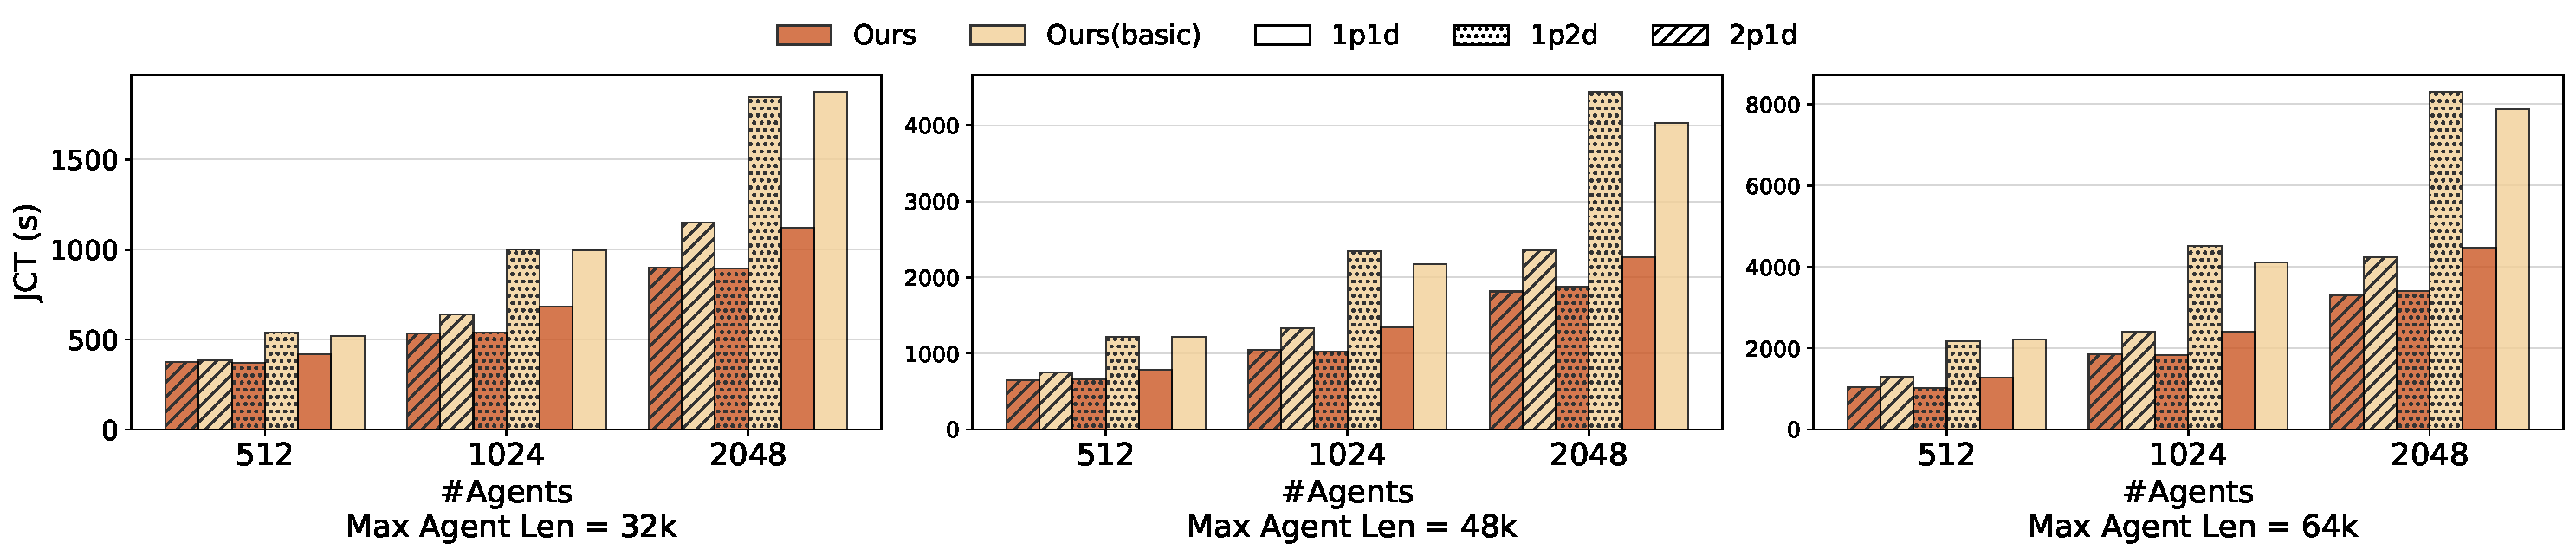
\includegraphics[width=\linewidth]{figures/27b_rollout_diffpd}\\
  \caption{\normalfont Impact of prefill-decode ratio on offline inference performance (DS 27B).}
  \label{fig:rollout_diff_pd}
\end{figure*}



\begin{figure}[t]
  \centering
  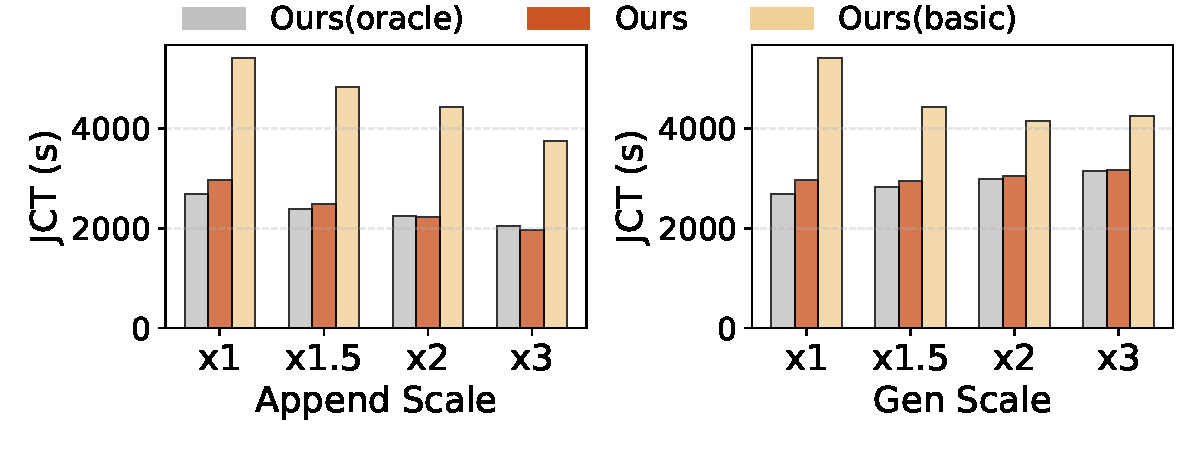
\includegraphics[width=\linewidth]{figures/660b_rollout_var_append_64k_traj512}
  \caption{\normalfont Left: varying append lengths (DS 660B, 64K context, 1024 agents). Right: varying generation lengths (DS 660B, 64K, 1024 agents)}
  \label{fig:rollout_diff_append}
  \end{figure}




\begin{figure*}[htbp]
  \centering
  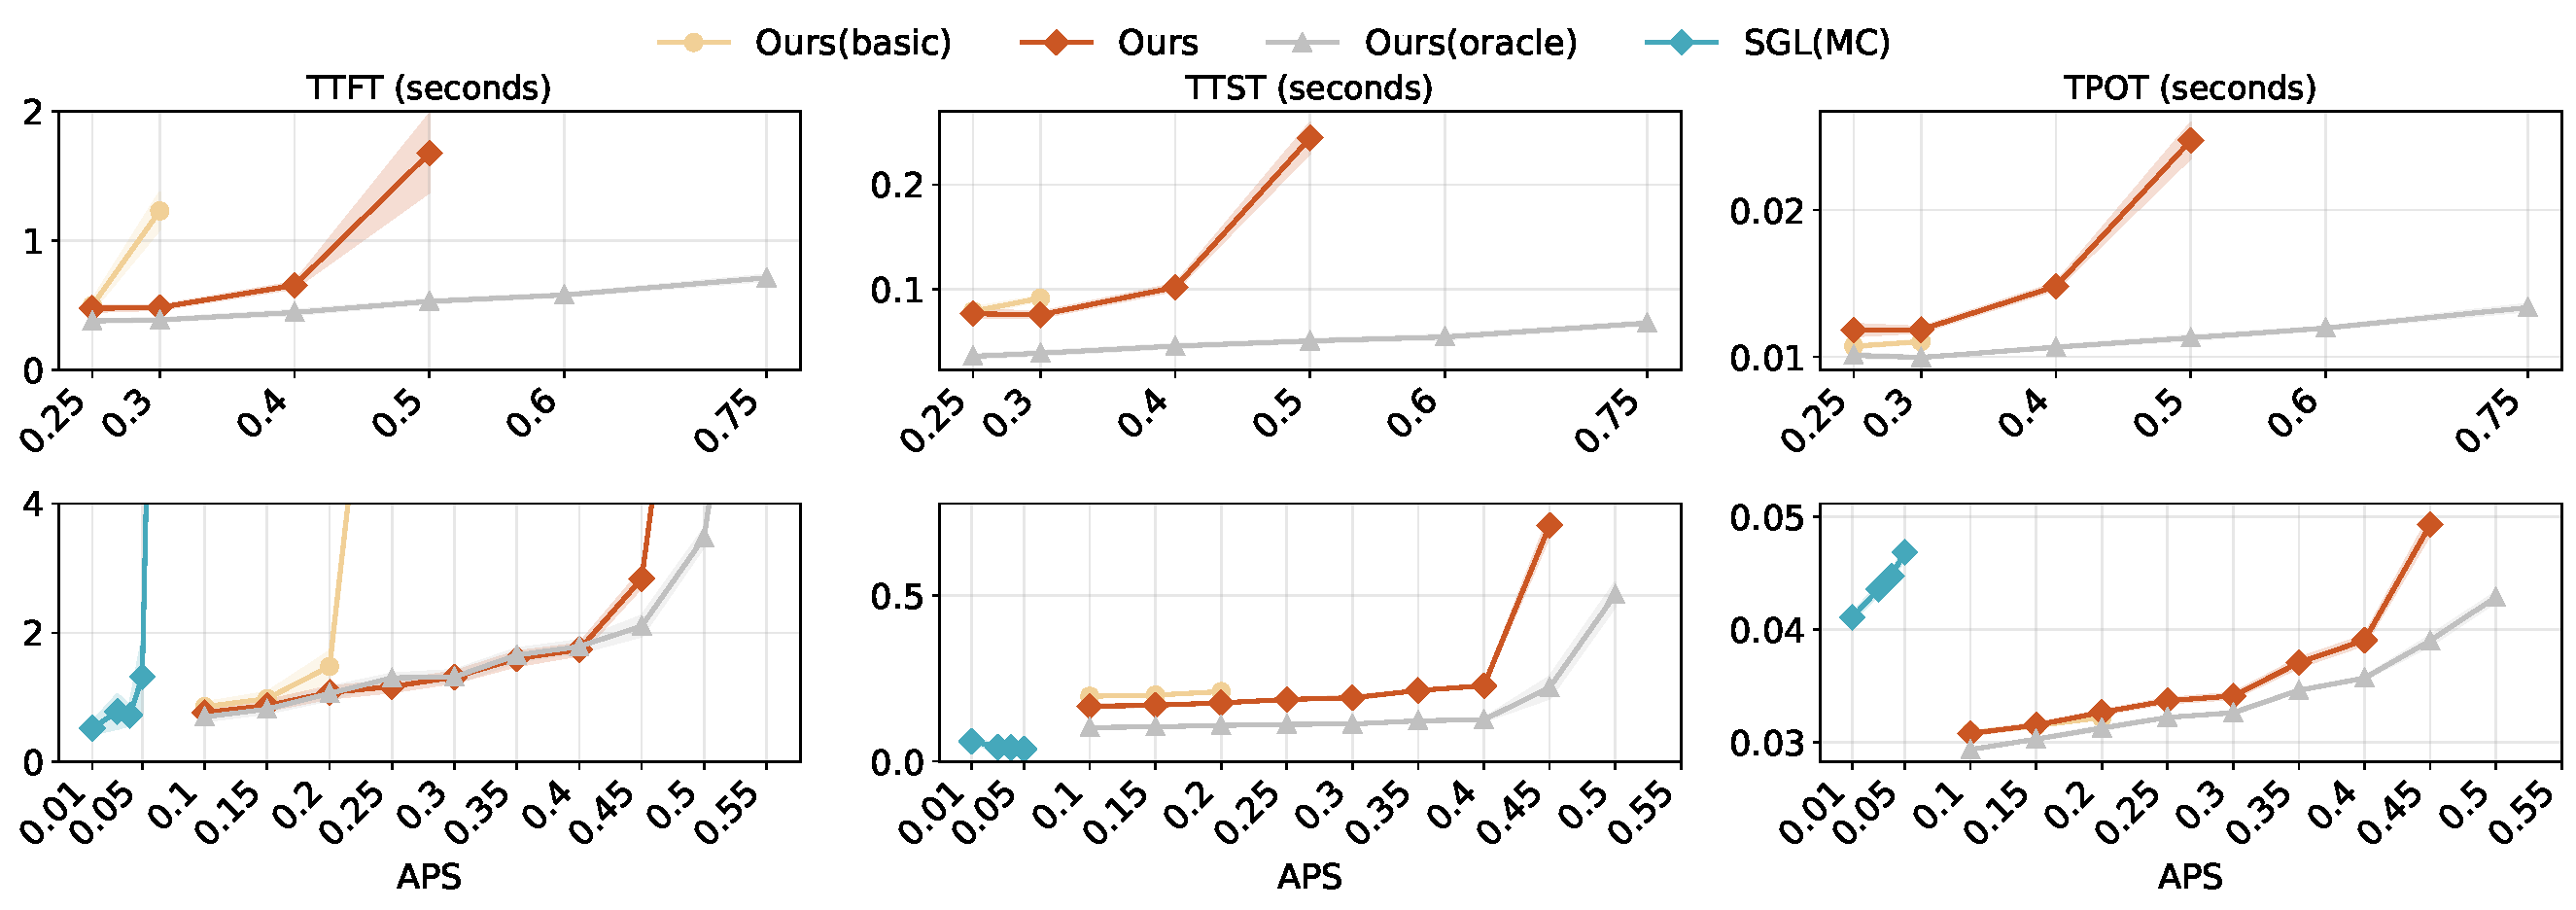
\includegraphics[width=0.88\linewidth]{figures/660b-27b-serving-aps-ttft-ttst-tpot}
  \vspace{-2mm}
  \caption{\normalfont TTFT, TTST, and TPOT as functions of agent arrival rate (APS). Shadow means the fluctuation in the last 150s before experiments finish. Top: DS 27B, Bottom: DS 660B.}
  \label{fig:serving}
\end{figure*}

\parabf{Varying Append Length \& Generation Length.}
\sysname has more advantages when append and generation tokens are short.
Longer append lengths imply greater GPU compute pressure, and longer generation lengths lower KV-Cache loading pressure due to larger prefill gap time.
To investigate the impact of this factor, we scale each round's append length by a constant factor, and then truncate the whole trajectory at given MAL.
The same holds for generation length.
As shown in \autoref{fig:rollout_diff_append}, with append length increases, Basic performance gradually approaches \sysname and Oracle, while \sysname and Oracle performance changes only slightly, indicating that the bottleneck consistently lies in GPU compute pressure.
Compared to Basic, \sysname achieves $1.82-1.99\times$ speedup at different append scales.
The trend for generation length scaling is similar.




\parabf{Varying Prefill-Decode Ratio.}
Across all ratios, \sysname demonstrates substantial performance gains compared to Basic.
We conduct rollout experiments on DS 27B with 1P1D, 2P1D, and 1P2D prefill-decode ratios to characterize the impact of resource allocation between prefill and decode stages on overall system performance.
As shown in \autoref{fig:rollout_diff_pd}, \sysname achieves an average speedup of $1.64\times$ across all configurations (up to $2.46\times$).
Basic 1P1D and Basic 1P2D perform comparably; 
so do \sysname 1P1D and Basic 2P1D, 
as well as \sysname 2P1D and \sysname 1P2D.
This occurs because each pair of systems has equivalent available storage bandwidth (Basic can only use prefill node storage bandwidth, while \sysname can utilize all nodes), which confirms that storage bandwidth is the dominant bottleneck in agentic scenarios.



\subsection{Online Serving}
\label{subsec:online-serving}
\parabf{Methodology.} We evaluate system latency characteristics under varying agent arrival rates per second (APS).
Agents arrive according to a Poisson process at a specified rate, with each agent commencing replay from round zero to its last round upon arrival.
For our experiments, the SLO is set as TTFT $\leq$ 4 seconds and TPOT $\leq$ 50ms.
In the TPOT and TTST figures, data points exceeding the SLO threshold are omitted.
Experiment termination is triggered when either: (1) TTFT exceeds 4 seconds, or (2) the system reaches steady state, defined as TTFT variation within a 150-second sliding window remaining below 5\% compared to that 30 minutes prior. 



As shown in \autoref{fig:serving}, \sysname achieves higher APS capacity than Basic (1.67$\times$ for DS 27B, 2.25$\times$ for DS 660B).
\sysname's TTST is comparable to Basic, while TPOT shows that \sysname does not introduce additional decoding overhead compared to Basic.
SGL(MC) exhibits anomalously low TTST, likely due to implementation issues where the first two tokens arrive at the 
client almost simultaneously.
For DS 27B, all metrics exhibit trends similar to DS 660B.
However, both Basic and \sysname show significantly higher TPOT than Oracle, suggesting the overhead of basic P-D transferring is considerable in small model cases. We leave it as future work.


\begin{figure}[hbtp]
  \centering
  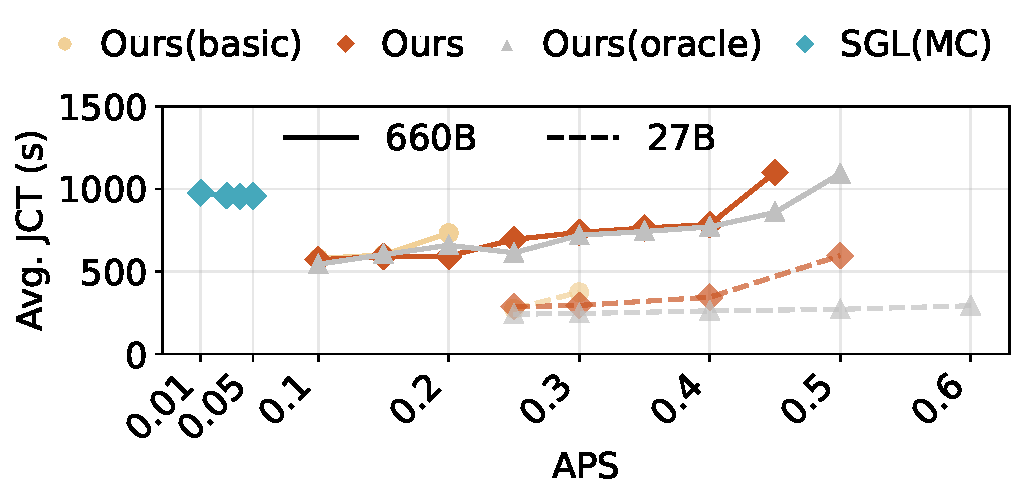
\includegraphics[width=0.9\linewidth]{figures/serving-aps-avg-jct}
  \vspace{-2mm}
  \caption{\normalfont Average completion time of all trajectories versus arrival rate for online serving.}
  \label{fig:serving-jct}
\end{figure}
Average JCT for both models are presented in \autoref{fig:serving-jct}.
A detailed analysis of working set implications is discussed in \autoref{sec:discussion}.
As shown in \autoref{fig:ablation-and-ttft-breakdown} (left), \sysname maintains stable TTFT components across different APS, while Basic's queuing time grows dramatically due to insufficient storage bandwidth.



\subsection{Ablation Study}
\label{subsec:ablation}



\begin{figure}[t]
  \centering
  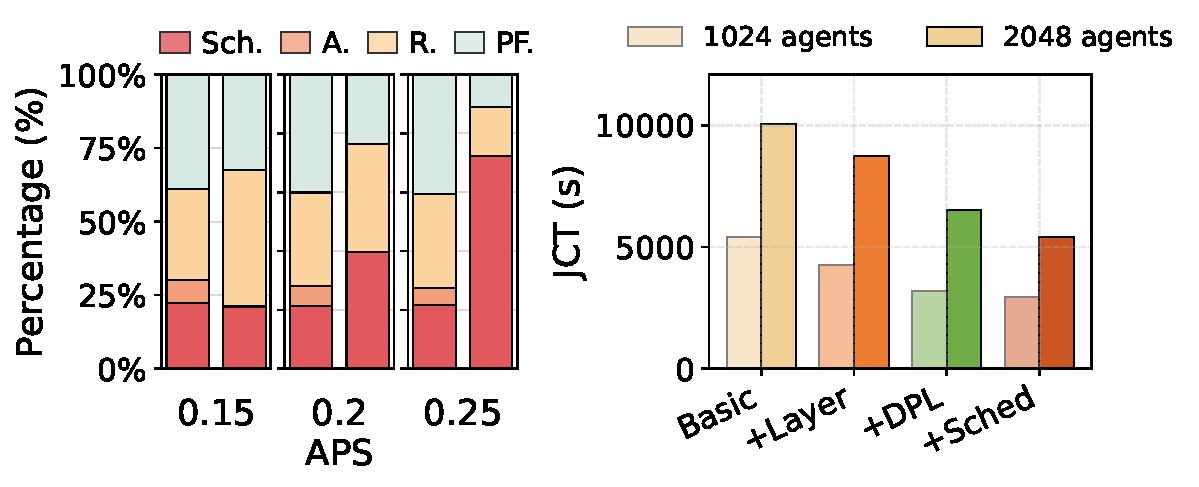
\includegraphics[width=\linewidth]{figures/660b_serving_breakdown}
  \caption{\normalfont Left (\autoref{subsec:online-serving}): TTFT breakdown for online serving (DS 660B) across APSs, Sch. for scheduling, A. for allocating, R. for reading KV-cache, PF. for prefill. In each pair of pillars, the first is for \sysname and the second is for Basic. Right (\autoref{subsec:ablation}): Offline inference ablation results (DS 660B, 64K context length). Layer, DPL, Sched stands for Layerwise prefill, Dual-Path Loading, and scheduling, respectively.}
  \label{fig:ablation-and-ttft-breakdown}
\end{figure}


We conduct an ablation study to quantify the contribution of each technical component in \sysname.
Experiments are performed under the offline inference setting with 64K MAL and agent batch size 1024 and 2048.
The differences between Basic and Ours are grouped into three techniques: layerwise prefill, dual-path loading, and scheduling algorithm. 
We add the techniques gradually to demonstrate individual contribution.
As shown in \autoref{fig:ablation-and-ttft-breakdown}, compared to Basic, adding layerwise prefill reduces JCT by $17.21\%$ on average, alleviating PE HBM bottlenecks and hiding transfer overhead.
Adding Dual-path loading on top of layerwise prefill delivers the primary performance gains, reducing JCT by $38.19\%$ on average compared to Basic, as it enables requests to read KV-Cache from either PE or DE, fully utilizing distributed storage bandwidth.
Finally, employing our scheduling algorithm on top of dual-path loading to decide KV-Cache loading paths achieves the best performance, reducing JCT by $45.62\%$ compared to Basic, demonstrating the effectiveness of load-balanced scheduling across storage NICs.



\begin{figure}[t]
  \centering
  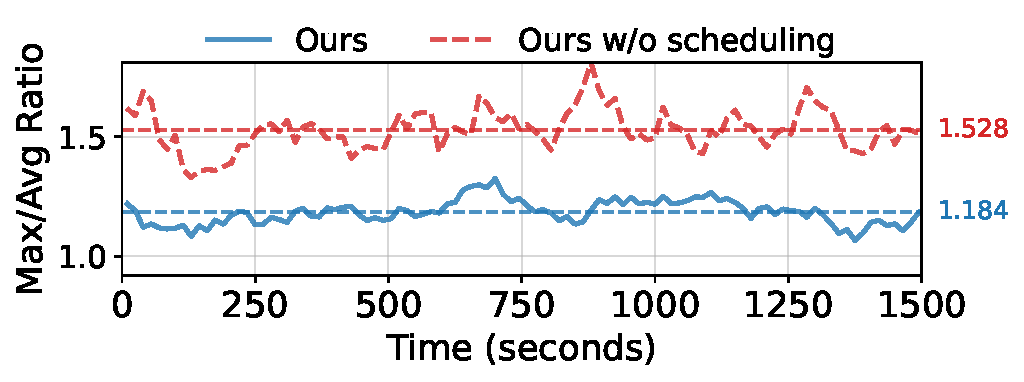
\includegraphics[width=0.9\linewidth]{figures/read_lb_48k_1024traj}
  \vspace{-3mm}
  \caption{\normalfont Load balance of storage NICs traffic}
  %  with 64k MAL, 1024 agents batch size.
  \label{fig:read-lb}
\end{figure}



\begin{figure}[t]
  \centering
  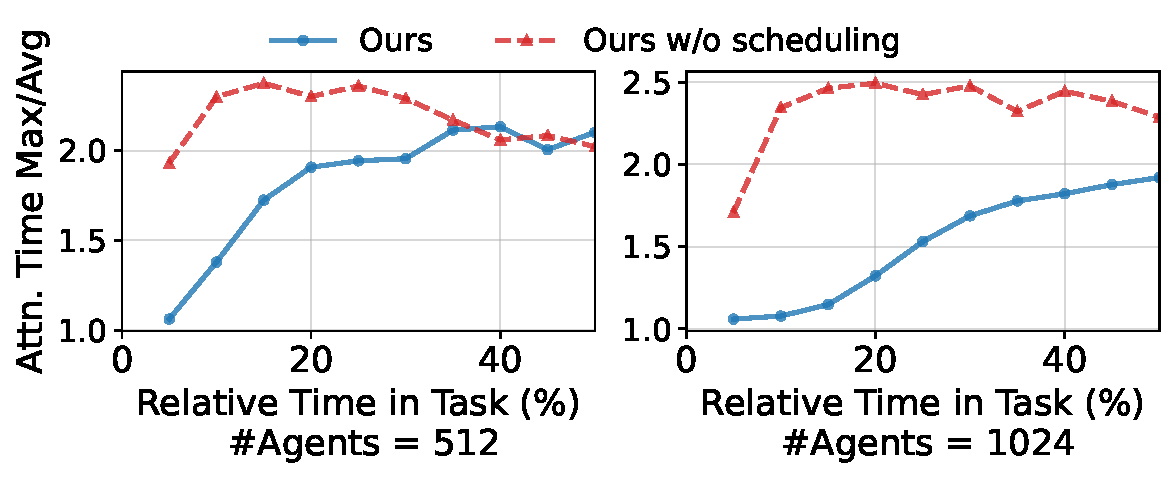
\includegraphics[width=\linewidth]{figures/attn_lb_48k}
  \caption{\normalfont Load balance of attention execution time.}
  \label{fig:attn-lb}
\end{figure}


\parabf{Load Balance.}
\sysname's scheduling algorithm improves load balance for both storage NICs and attention layer execution times.
For storage NICs, our scheduling algorithm improves load balance from 1.53 to 1.18 compared to round robin scheduling (\autoref{fig:read-lb}).
For attention layers, \sysname maintains the Max/Avg ratio as low as 1.06 during the first 5\% of the task, reducing GPU idle bubbles (\autoref{fig:attn-lb}).
The storage NIC metric is the ratio of maximum to average traffic across all storage NICs on three machines within a small time window, where 1.0 represents perfect balance.
The attention layer metric is calculated among all GPUs in an expert parallel group for each forward.
As the task progresses, both ratios become meaningless due to underloaded system. 
Therefore, we do not show the tail phase of the workload.




\begin{table}[t]
  \centering
  \caption{\normalfont Large-scale experiment results.}
  \label{tab:largescale}
  \setlength{\tabcolsep}{3pt}
  \small
  \begin{tabular}{cccccc}
  \toprule
  & \textbf{Setting} & \textbf{JCT} & \textbf{TTFT} & \textbf{TTST} & \textbf{TPOT} \\
  \midrule
  \multirow{2}{*}{\rotatebox{90}{\scriptsize Offline}} 
  & 2P4D, 2K agents & 3,167s & -- & -- & -- \\
  & 48P96D, 48K agents & 3,201s & -- & -- & -- \\
  \midrule
  \multirow{2}{*}{\rotatebox{90}{\scriptsize Online}} 
  & 2P4D, 0.4 APS & -- & 1.739s & 0.228s & 0.039s \\
  & 44P88D, 8.8 APS & -- & 1.847s & 0.194s & 0.036s \\
  \bottomrule
  \end{tabular}
  \end{table}

\begin{figure}[t]
  \centering
  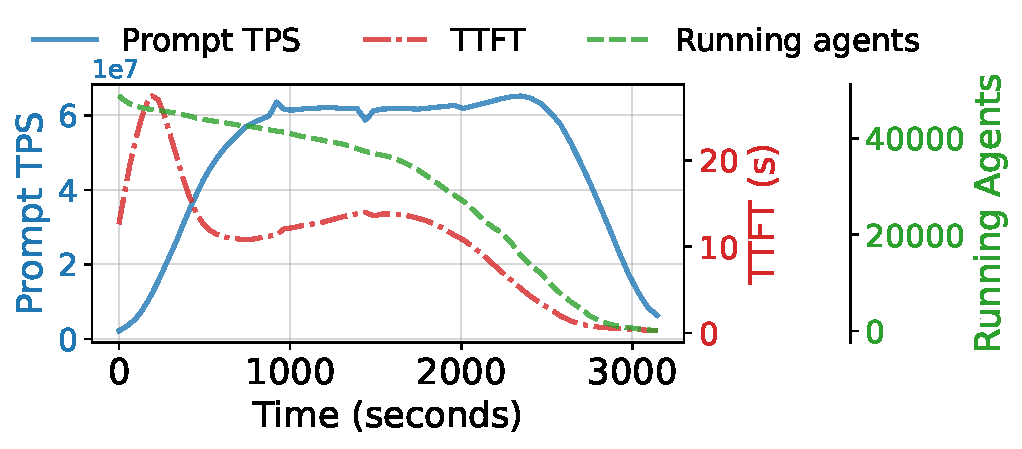
\includegraphics[width=\linewidth]{figures/largescale_rollout.pdf}
  \caption{\normalfont 48P96D offline inference metrics. 1e7 is the scaling factor of Prompt TPS.}
  \label{fig:largescale-rollout}
\end{figure}

\subsection{Large-Scale Scalability}



We conduct both offline and online experiments using up to 1,152 GPUs to demonstrate large-scale scalability (\autoref{tab:largescale}). 
For offline inference, scaling from 2P4D (2K agents) to 48P96D (48K agents) achieves near-linear speedup with comparable JCT (3,167s vs.\ 3,201s). 
For online serving, the 44P88D configuration achieves 22$\times$ throughput (8.8 vs.\ 0.4 APS) while maintaining similar latency. 
Across all experiments, scheduler CPU usage remains below 10 cores, confirming it is not a bottleneck. Some detailed metrics over offline inference process are shown in \autoref{fig:largescale-rollout}.

Due to the lack of fine-tuned parallelism settings and P/D ratios (which requires a substantial experimentation budget), the large-scale experiments do not demonstrate additional JCT or serving capacity gains compared to multiple small-scale units with equivalent cost.
However, large-scale setting remains important for the following reasons. First, it reduces fragmentation and provides greater flexibility for fine-tuning parallelism and P/D ratios. Second, large-scale deployment offers more scheduling opportunities to mitigate queuing latency under unpredictable bursty online requests. These observations suggest several directions for future work (\autoref{subsec:futurework}).

